\chapter{Model-View-Controller for Science}\label{ch:mvcs}

\section{Introduction}\label{sec:mvc-introduction}
Developing a computer program is much more than having a few scripts that we can run when we need them. The software should take care of a lot of concerns, such as the limits of the devices, should be flexible enough that enables you to change what measurements you are doing without spending months. More importantly, a program should be extensible in the long run, not just by yourself but also by future colleagues and, potentially, by anyone who finds your application online.

Therefore, when we develop software, we want to keep in mind the following programmer's \emph{mantras}:

\begin{itemize}
\item What you develop should be readable by current and future colleagues
\item It should be easy to add solutions developed by others
\item The program should allow exchanging devices that achieve the same goal (e.g., oscilloscopes of different brands)
\item The code developed in one context has to be available in other contexts (i.e., in other experiments)
\end{itemize}

The first line does not pose a challenge to be understood. When we talk about solutions developed by others, we mean that often someone already wrote a driver for a device, or they wrote a measurement script. Therefore, it should be easy to get other's code and use them in our projects. Exchanging hardware is something that is not valued until it happens. In most labs, there is always a legacy device that sooner or later breaks down, and we need to replace it. Or you move to a different lab and need to continue with your experiments with different hardware. There are patterns that we can follow to allow a simple exchange of devices. Finally, when we talk about context, we mean that sometimes experiments are very different, but the logic behind it is very similar. We measure the I-V curve of a diode, but it is, by no means, any different from doing a 1-D scan on a confocal microscope, or tuning the wavelength of a laser.

The mantras are no rules. They are just points on which you have to reflect on realizing whether you are departing from the path you wanted to follow when you started. In the following sections, we are going to explore a design pattern for software that has many benefits when developing scientific software for controlling experiments. It is called \textbf{The Model-View-Controller for Science}

\section{The MVCs design pattern}\label{sec:mvc}
\begin{center}
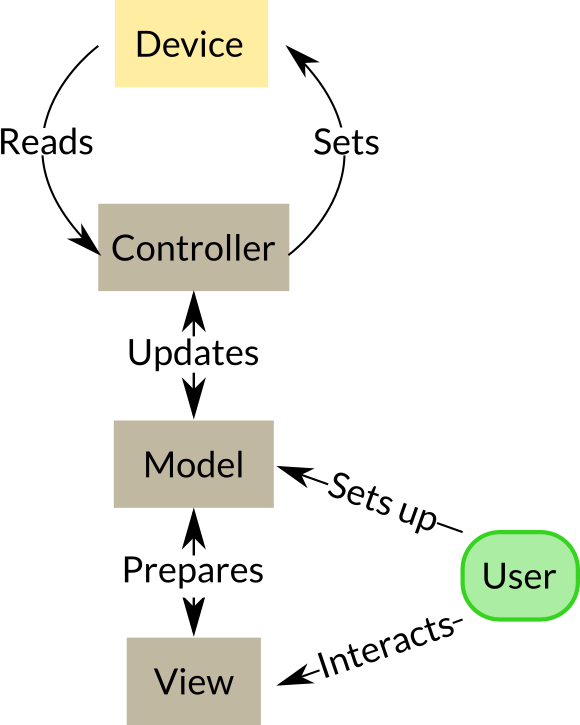
\includegraphics{images/Chapter_04/MVCs.png}
\end{center}

A design pattern is nothing more than a set of rules that determine where we can place different parts of the code and how they are going to interact with each other. One of such patterns is called the Model-View-Controller, or MVC for short. When you work with devices in the lab, there is an extra layer that most computer programs lack, which is the interaction with the real world through specific devices. That is why we decided to nickname the pattern MVCs, with the s for \emph{science}. Let's see what each component of the MVC is.

A \emph{Controller} for our purposes can also be called \emph{a driver}, which is responsible for communicating with devices. It can be a Python class we developed ourselves, such as the one we did in the previous chapter, but it can also be a Python package developed by someone else. The latter scenario is the case when manufacturers provide the drivers themselves, such as PyPylons from Basler, or the NI-DAQmx bindings for Python. The driver has to reflect the capabilities of the device, nothing less and nothing more. For example, if a device can acquire just a data point at a time, the driver shouldn't include a function for acquiring an array of data using a loop. We briefly discussed this in the previous chapter. Whatever belongs to the logic that a user imposes belongs to the Model component.

The \emph{Model} is where all the logic is defined. In the models, we are going to determine how we are going to use a device for our experiment. A clear example would be the introduction of units. The Device class from the previous chapter takes only integer values as arguments of the methods. If we would like to transform that information into voltages, we could do it in the model.

Moreover, in the experiment itself, we measure voltage, but we can convert it into a current with Ohm's law. This behavior is particular to our experiment, and thus the option shouldn't be hardcoded in the driver. The place to include this information is the Model. The main advantage of splitting \emph{Controllers} and \emph{Models} is that it becomes simple to upgrade or replace a device. You need to update the \emph{Model} to reflect the new options of the device, but the logic of the experiment is left intact.

There is a second type of model, which is the \emph{Experiment Model}, in which we link different devices to perform a measurement. Or we use a single device, but we add the features that an experiment needs, for example, saving data, plotting, analyzing, transforming units. With straightforward cases, the boundary between the device model and the experiment model can be blurry. Still, when you are dealing with several devices or more complex flows, it becomes much clearer. At the end of the book, we give a reference to some projects we have worked on, which can be a good source of inspiration.

The \emph{View} is the place where you can locate everything related to how you show data to the user and how the user can change the parameters of the experiment. In practice, it is the collection of files that build up a Graphical User Interface ({GUI}). Within the {GUI}, you set, for example, the start, stop, and step of the experiment. This information is passed to the model to acquire the data, save it, and plot it. We must note, however, that the user interacts through the View with the Model, but never directly with the Controller. It is also essential to keep in mind that we implement all the logic in the Model. For example, if we save the data to files, the procedure to create new filenames should be specified in the Model and not in the View.

For our project, the controller is what we discussed on Chapter~\ref{ch:first-driver}, the model for the device will be discussed on Chapter~\ref{ch:device-model}, the model for the experiment on Chapter~\ref{ch:experiment-model}, and the view will be discussed in Chapters~\ref{ch:starting-gui} and~\ref{ch:user-input-designer}. As you can see, there are still many things to cover in the book. It is important to be patient, because we are going to grow a solution slowly, based on need, and solving the mistakes that may appear as we go, and not just following a path blindly.

\tipsInfo{Why Splitting the Code}{For people who are new to developing code for the lab, it may be hard to understand why and how to split \emph{Controller} and \emph{Model}. When you have only one device that you use for only one goal, and that is as simple as the device we are using in this book, the differences between model and Controller are very thin. However, when you wish to include code developed by others or when you want to share your code, it is crucial to split the capabilities of your device from the logic of your experiment. If you don't do so, all your code is going to work when doing just one particular experiment.}

The meaning of \emph{Model}, \emph{View} and \emph{Controller} changes depending on each developer or community. People developing a web application are not dealing with devices in the real world as developers in the lab do. Therefore, the {MVC} pattern definition can change from one field to another. The details are not that important; once we establish a structure, if we follow it, everyone else will be able to understand quickly what the code is doing and where. Once we understand what each different component is, we will very quickly understand where we need to change the code to solve a bug or add new functionality.

\section{Structure of The Program}\label{sec:structure-of-theprogram}
In the program we are developing in this book, we follow the MVC design pattern quite literally. This means that we have to create three folders called \emph{Model}, \emph{View} and \emph{Controller}. In the previous chapter, we have already developed the driver for the device. Go ahead and move the file \textbf{pftl\_daq.py} into the Controller folder.

\questionInfo{Exercise}{Create a file \textbf{analog\_daq.py} in the Models. Inside the file, define a class called \mintinline{python}{AnalogDaq} what methods do you think that belongs to the device Model?}

In our definition of Model, it is vital to make a further distinction. On the one hand, we have models for the devices we use. In those models, we define things such as units, or how to initialize the device. However, experiments often require to perform complex tasks in which we need to synchronize several instruments. When we perform a measurement, we need to save the data or load the configuration from a file.

\questionInfo{Exercise}{Create a file in the Models folder, called \textbf{experiment.py}. Define a class called \mintinline{python}{Experiment} and add some methods that you think are going to be useful. You can, for example, add a method for switching on or off the {LED}. You can also add a method for doing a scan of an analog output signal. The methods can be empty, don't worry about making it work, but just about the layout. You have to start thinking about the parameters that you need and the order in which you can call every method. For example, to save the data, you need to specify a folder first.}

The View folder is going to require a bit more of work than the other two. However, you can already start thinking about how the user is going to interact with your program. Most likely, you have thought that sometimes the {LED} will be plugged into the output channel number 1, sometimes to channel number 0. You don't want to change the code every time you change where you connected the LED. The same happens, for example, with the channel you want to monitor, or the time delay between steps. We include all this behavior in the View that we develop in the last chapters of the book.

Now that you have started to split the code into different folders and files, it is essential to discuss how you can make programs that use the code available in separate files. That is called \emph{importing} and is the focus of the next section.

\section{Importing modules in Python}\label{sec:importing-python}
In the previous chapter, we have already seen some lines that look like this:

\begin{minted}{python}
import numpy as np
from time import sleep
\end{minted}

The first one is importing the numpy package, but changing its name to \mintinline{python}{np}. Changing the name makes it easier to work with because you need to type only two letters, \mintinline{python}{np} instead of \mintinline{python}{numpy}. The second line is importing one specific function from a package called \mintinline{python}{time}. It is important to realize that the import process was different in both cases. \emph{Numpy} is a complex package, with many modules that we can use. The same is true for \emph{time}. However, in the lines above, we have imported only the module \emph{sleep} from package \emph{time}. If we want to use it, we can do:

\begin{minted}{python}
sleep(1)
\end{minted}

While for using \emph{Numpy}, we will need to specify which module we want:

\begin{minted}{python}
np.random.random(1)
\end{minted}

If we know we only want to use \mintinline{python}{random} from \emph{Numpy}, we can also import and use it like this:

\begin{minted}{python}
from numpy.random import random

random(1)
\end{minted}

We may wonder why we would import all of numpy is you are just using one of its functions. The name \emph{random} is not defined solely by numpy. Python also provides its random module. We can import it like this:

\begin{minted}{python}
import random
\end{minted}

If we needed both \emph{random} functions in the same program, we would have a clash. How would we be sure we are using Numpy's and not Python's function? We may, for example, define our random function, and we would like to be able to choose which one to use and, more importantly, we want to avoid generating an unexpected behavior because of redefining functions without realizing it.

When working with our code, we can import different modules in the same way. Open a terminal and navigate to the root folder of the project, i.e., the folder that contains the Model, View, and Controller folders. Start the Python interpreter, and then type:

\begin{minted}{pycon}
>>> from Controller.pftl_daq import Device
\end{minted}

Now we have the controller available to use. We can do the following:

\begin{minted}{pycon}
>>> dev = Device('/dev/ttyACM0')
>>> dev.initialize()
\end{minted}

However, there is something strange happening if we run the code above. As soon as we import \py{Device}, it starts communicating with the device, outputs the identification number, and switches on and off the LED. This behavior is, of course, something we don't want, and a very common pitfall for Python developers. Of course, we don't want to trigger a measurement just because we imported the module to our program.

To avoid running code when importing, we must change the file \textbf{pftl\_daq.py}. We can add one line of code at the end of the file, and some indentation, to make it look like this:

\begin{minted}{python}
if __name__ == "__main__":
    dev = Device('/dev/ttyACM0') #<---- Remember to change the port
    dev.initialize()
    serial_number = dev.idn()
    print(f'The device serial number is: {serial_number}')
    for i in range(10):
        dev.set_analog_output(0, 4000)
        volts = dev.get_analog_input(0)
        print(f'Measured {volts}')
        sleep(.5)
        dev.set_analog_output(0, 0)
        volts = dev.get_analog_input(0)
        print(f'Measured {volts}')
        sleep(.5)
\end{minted}

To see the changes, we first must close Python running the \py{exit()} command, and then opening it again. Python does not import twice the same modules, and therefore, it won't realize that the file with our Controller changed. After we restart Python, we can try again importing the Controller. Now things are going to look fine, and we can use the \py{Device} as we intended. We can leave the space at the bottom of files to hold examples of how to use the code above. If we ever find the Device around, and we don't remember what we were supposed to do with it, we can always go to the bottom of the file and see how it works.

Every time we encounter a behavior which is not easy to understand, the best idea is to transform it into simpler components and explore them one by one. In this case, the importing process may be a bit confusing. To understand it a bit more about, especially how the \mintinline{python}{if __name__} works we can create a new file called \textbf{dummy\_controller.py} in the \emph{Controller} folder, with the following lines of code:

\begin{minted}{python}
print('This is the dummy Controller')

def dummy_example():
    print('This is a function in the dummy Controller')

if __name__ == '__main__':
    print('This is printed only from __main__')
    dummy_example()

\end{minted}

From the Terminal, we can just type \py{python Controller.dummy_controller.py}. The output should be:

\begin{minted}{bash}
This is the dummy Controller
This is printed only from __main__
This is a function in the dummy Controller
\end{minted}

What we see is that the entire code got executed.

\questionInfo{Exercise}{What do you expect to happen if you do \mintinline{python}{import dummy_controller}?}

Things are going to be different when we import the file. In the Python interpreter we can do the following:

\begin{minted}{pycon}
>>> from Controller import dummy_controller
This is the dummy Controller
>>> dummy_controller.dummy_example()
This is a function in the dummy Controller
>>> from Controller.dummy_controller import dummy_example
>>> dummy_example()
This is a function in the dummy Controller
\end{minted}

First, we notice that the code at the end never gets executed. This means that the \py{if} statement is not \py{True}. This block is handy when we want to have code that works standalone (when we execute it directly, for example), but we don't want to execute those lines if we import it. In the case of the real Controller, we wanted to leave some examples at the end to show how we can use it, but when we are importing a class, we don't want it to start communicating with the device.

We can also see that the line \py{"This is the dummy Controller"} appears only once. Python knows that we have already imported the module \textbf{dummy\_controller}, and it doesn't execute again the lines that we already imported. Therefore, we have to be aware that it is not a matter of using the \py{from} in the importing procedure. We can close Python, start it again and revert the order in which we import, and the print is still there the first time but not the second. It means that Python is smart when importing modules, and won't fetch the elements it already has available, even if we are importing in a slightly different way.

\tipsInfo{Naming Conventions}{We should establish some naming conventions to avoid confusion later on. In Python, any file that defines variables, functions, or classes is called a \mintinline{python}{Module}. The folder that contains modules is called a \mintinline{python}{Package}.}

Working with the imports in Python is sometimes easier than understanding them, especially when trying to pay attention to all the different definitions. The Python Documentation\footnote{https://docs.python.org/3.6/tutorial/modules.html} has an excellent chapter covering a lot of the ideas discussed. Many of the properties and behaviors can be learned by trial and error, though it can be very time consuming, and it may lead to unexpected errors.

There is one final remark that is worth mentioning about packages. Right now, we have three folders in our project: Model, View, and Controller. But what would happen if we add a new folder called, for example, \emph{serial}? Next time we try to do \py{import serial}, how would Python know if it is supposed to import the PySerial library or our package? It can also happen the other way around, perhaps we don't know there is something already called \emph{Controller} in Python, and we don't care about it, we want to import our modules.

For Python to understand that a folder is a \emph{package}, we should add an empty file called \textbf{\_\_init\_\_.py}. This file is the way of letting Python know that a folder is more than a plain directory, and thus it should be treated like that. Therefore, we must add the empty init files in the three folders we have created so far. If you are using a Python IDE, such as Pycharm, you notice that these files get created automatically if you chose 'new package' while trying to add a folder.

\questionInfo{Exercise}{Create a folder called \textbf{random} and inside create a new file called \textbf{test.py}. Define a function inside the file. It is not important what it does, and then you save it. Start Python and see what happens if you do \mintinline{python}{from random import test}. Quit the interpreter and add an empty file called \textbf{\_\_init.py\_\_} inside the \textbf{random} folder. Try to import \textbf{test} again and see what happens.}

The init files of packages allow us to specify more complex behaviors when importing, but that goes beyond the scope of this book. Going through other packages is an excellent way of understanding how developers have decided to structure their code.

\section{The PATH variable}\label{sec:path}
There is still a huge difference between our code and the way a library, such as \emph{Numpy}, can be imported. \emph{Numpy} can be imported regardless of where we have started the Python interpreter. We can go to any folder in the Terminal, start Python and import numpy. However, we can import our package only if we are in its directory. If we are sitting on a different folder and try to import the Controller, we get an error like the following:

\begin{minted}{pycon}
>>> from Controller.pftl_daq import Device
Traceback (most recent call last):
  File "<stdin>", line 1, in <module>
ModuleNotFoundError: No module named 'controller'
\end{minted}

Python searches for packages in specific locations, and once it finds one, it stops searching. \emph{Numpy} is located in one of the folders that Python uses, but Python is not aware of our package yet. One way to let Python know where our package is located, is by adding the folder to a system variable called \emph{PYTHONPATH}.

On Windows, we can follow the steps explained in Section~\ref{subsec:path-windows}, when we were dealing with the details of adding environment variables after installing Python. The only difference is that we should use the variable PYTHONPATH instead of just PATH. On Linux, it is enough to run the following command:

\begin{minted}{bash}
$ export PYTHONPATH=$PYTHONPATH":/path/to/PFTL"
\end{minted}

We have to change \py{/path/to/PFTL} with the full path to the folder where we are keeping the code. After doing that, we can type \py{from Controller import *} wherever you are in your computer, and Python finds the appropriate folder. On Linux, the change is not permanent, and we need to rerun the line next time we start the Terminal. We can modify environment variables permanently, but this goes too much into the details of the operating systems.

If you are using an IDE to develop and run the code, you may have noticed that there is no need to add anything to the Python path. It is one of the advantages of using robust programs to develop software. They take care of many things for us. However, at some point, it is also essential to be able to run the program independently of the editor software.

\section{The Final Layout}\label{sec:final-layout}
At this stage, we should have a clear separation of the code into Model, Controller, and View. Most of them are, for the time being, empty folders. However, we are not limited to having only three folders in our project. Most likely, we want to provide some examples of how to use the code or some documentation.

However, if we create extra folders next to the three main ones, the structure of the program starts to be polluted. It won't be clear what is part of the program, and what is a user-specific setting. Therefore, it is a common practice to make a folder to hold all the program and, next to it, we create an extra folder to contain non-essential elements. In our case, the folder structure would look like this:

\begin{minted}{text}
├── Docs/
├── Examples/
└── PythonForTheLab/
    ├── Controller/
    │   ├── __init__.py
    │   └── pftl_daq_01.py
    ├── Model/
    │   └── __init__.py
    ├── View/
    │   └── __init__.py
    └── __init__.py
\end{minted}

There are three folders at the top level: \emph{Docs}, \emph{Examples} and \emph{PythonForTheLab}. The last one is holding the \emph{Model}, \emph{View} and \emph{Controller} with all the code that you have developed up to now. The \emph{PythonForTheLab} also requires an \textbf{\_\_init\_\_.py} file, because it is our main package. This folder structure would allow us to do the following:

\begin{minted}{pycon}
>>> from PythonForTheLab.Controller import pftl_daq
\end{minted}

This code is clearer than importing the Controller directly, because it also allows us to, in principle, have different programs at the same time and import only the elements we need from each one. For example, we could have one big project with many devices and complex measurements, and a smaller program to do more specialized tasks that only require \emph{some} of the devices.

\section{Conclusions}\label{sec:layout-conclusions}
Following a pattern when programming makes the code much easier to understand, to maintain, and to explain to others. Patterns, however, are not set in stone. Sometimes there is no clear divide between what we should develop where. The important thing is to be consistent. For example, if at some point it is decided that controllers should handle real-world units, then all controllers should do it. If, on the other hand, we agreed that models should handle units, then all models should do it, regardless of what the specific controllers do.

Following a pattern is useful not only when there are many developers involved in the same project, but also when the same person is working on different projects, or if they change labs, or experiments. As time passes, we start accumulating a collection of tools, and being able to transfer them from one experiment to another makes it much faster to have a measurement running without reinventing the wheel over and over again.

Another essential aspect for many scientists is that solutions should be developed as quickly as possible to test out new ideas. And this is how we laid out this book. First, we quickly manage to communicate with the device. We saw we can acquire data, switch on and off the LED. If the measurement would be a one-off task, then we would have finished. But if we would like to start changing parameters, or using the code for another experiment, then we must keep going. Expanding the code is what we are going to do next. In these sections, we have explored a sustainable way of following the \emph{Onion Principle}. Factoring also concerns about the speed at which we can implement a solution for the lab.

The strategies proposed in this chapter do not come naturally to every developer, and even if you know them, you can try to find shortcuts. The truth is that no one does an experiment only once. The key to better science is reproducibility, and the clearer the code that enabled you to acquire data, the easier it is to repeat a measurement, even by someone else. We can only lay out the foundations for what we consider a robust solution. If you find a different path, you are always free to follow it, but never miss the bigger picture from your sight.
